\documentclass[border=1mm]{standalone}

\usepackage{import}
\subimport{../../../}{preamble.tex}

\usepackage{tikz}
\usetikzlibrary{calc}
\usepackage{pgfplots}

\newcommand{\convexpath}[2]{
  [   
  create hullcoords/.code={
    \global\edef\namelist{#1}
    \foreach [count=\counter] \nodename in \namelist {
      \global\edef\numberofnodes{\counter}
      \coordinate (hullcoord\counter) at (\nodename);
    }
    \coordinate (hullcoord0) at (hullcoord\numberofnodes);
    \pgfmathtruncatemacro\lastnumber{\numberofnodes+1}
    \coordinate (hullcoord\lastnumber) at (hullcoord1);
  },
  create hullcoords
  ]
  ($(hullcoord1)!#2!-90:(hullcoord0)$)
  \foreach [
  evaluate=\currentnode as \previousnode using \currentnode-1,
  evaluate=\currentnode as \nextnode using \currentnode+1
  ] \currentnode in {1,...,\numberofnodes} {
    let \p1 = ($(hullcoord\currentnode) - (hullcoord\previousnode)$),
    \n1 = {atan2(\y1,\x1) + 90},
    \p2 = ($(hullcoord\nextnode) - (hullcoord\currentnode)$),
    \n2 = {atan2(\y2,\x2) + 90},
    \n{delta} = {Mod(\n2-\n1,360) - 360}
    in
    {arc [start angle=\n1, delta angle=\n{delta}, radius=#2]}
    -- ($(hullcoord\nextnode)!#2!-90:(hullcoord\currentnode)$) 
  }
}


\begin{document}

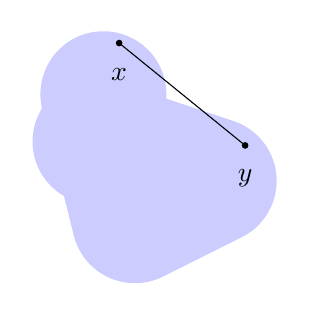
\begin{tikzpicture}[every node/.style={circle}]
  \node at (0,0) (a) {};
  \node at (1.5,-0.5) (b) {};
  \node at (0.5,-1) (c) {};
  \node at (0.1,0.6) (d) {};

  \fill[fill=blue!20] \convexpath{a,b,c,d}{0.8cm};

  \node[circle, fill=black, inner sep=0.3mm] at (0.3, 1.25) (x) {};
  \node[circle, fill=black, inner sep=0.3mm] at (1.9, -0.05) (y) {};
  \node[below] at ($(x)-(0, 1mm)$) {$x$};
  \node[below] at ($(y)-(0, 1mm)$) {$y$};

  \draw (x.center)--(y.center);
  
\end{tikzpicture}

\end{document}

%%% Local Variables:
%%% mode: latex
%%% TeX-master: t
%%% End:
